\section{Introduction}
\nblink{brats/12\_rise\_masks.ipynb}

The results from applying RISE on our segmentations problems (BraTS and testnet) where underwhelming. While they showed a low resolution heat map output on both tasks,
on the testnet is missed out a big part 

Heavily modified \cite{zeiler2014visualizing} and 
Prediction Difference Analysis \cite{zintgraf2017visualizing}


\begin{figure}[H]
    \centering
    \begin{subfigure}[t]{.32\textwidth}
        \centering
        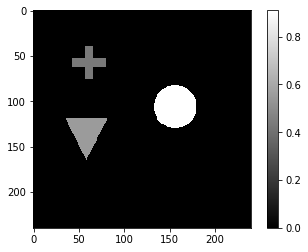
\includegraphics[width=\linewidth]{chapters/02_methods/images/rise/rise_original.png}
        \caption{Original image}
    \end{subfigure}\hfill%
    \begin{subfigure}[t]{.32\textwidth}
        \centering
        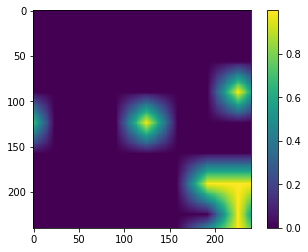
\includegraphics[width=\linewidth]{chapters/02_methods/images/rise/rise1_mask.png}
        \caption{RISE mask}
    \end{subfigure}\hfill%
    \begin{subfigure}[t]{.32\textwidth}
        \centering
        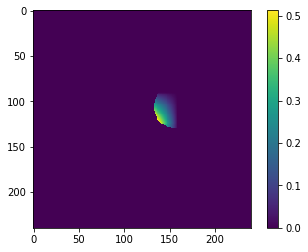
\includegraphics[width=\linewidth]{chapters/02_methods/images/rise/rise1_applied.png}
        \caption{RISE mask applied to original image by multiplication}
    \end{subfigure}
    \caption{By multiplication the input image (left) with a RISE mask (center), a modified input is generated (right).}
    \label{rise_mask0}
\end{figure}